\section{实验内容}

这一节将会对RFF的有效性进行实验来证明。作为一个基于模糊测试的并发漏洞挖掘工具,我们将RFF应用于真实世界的软件,来测试它挖掘漏洞的能力,同时还一些测试集上,对它进行测试以证明它对于各种并发漏洞的有效性。同时,我们还将RFF和之前的一些工作进行对比,以证明RFF能够比它们更有效的挖掘漏洞。最后,我们还将证明reads-from relation以及抽线调度对于RFF挖掘并发漏洞是有帮助的。

主要探究的问题有以下几个

\begin{enumerate}
\item RFF是否能够比其他现有的工具更加有效地发现漏洞
\item 抽象调度空间对于RFF有效性地贡献
\item RFF在reads-from空间中的探索的分布
\end{enumerate}

\subsection{实验配置}

\paragraph{基准}实验基于两个基准测试。分别是SCTBench和ConVul。选择这两个基准测试的原因是他们能够覆盖大多数的情况,包括漏洞的类型、软件的种类等。SCTBench结合了之前一些其他的基准测试,包括压缩工具,web引擎,并行数值计算等方面的软件。这些各种各样的软件,均利用了多线程的机制,其中不乏有超过几千行代码的软件,这些软件利用多线程的机制实现了复杂的操作,其中存在着并发漏洞。当工具对这些程序进行测试的时候,需要在复杂的代码逻辑中找到漏洞的位置,这对于工具的有效性提出了很高的要求,进而可以测试工具在挖掘并发漏洞方面的有效性。ConVul基准测试则包含了十个真实世界应用程序的并发漏洞。

\paragraph{对比工具}为了将RFF和当前最先进的并发漏洞测试工具进行相比较,实验将RFF和PERIOD,PCT ,GenMC进行了比较。其中,PERIOD通过将多线程程序进行关键点切片,系统地对并发访问空间进行探索,同时利用linux的基于deadline的任务调度机制,实现了可控的多线程调度。PCT利用了随机的算法生成特定深度的调度来测试程序,保证了检测到并发漏洞的最小概率。一些其他的模糊测试工具例如MUZZ和CONZZER,由于无法得到源代码或进行复现,我们没有将其作为基准测试一起进行比较。

\subsection{和当前先进的工作进行比较}

\begin{figure}[ht]
    \centering
    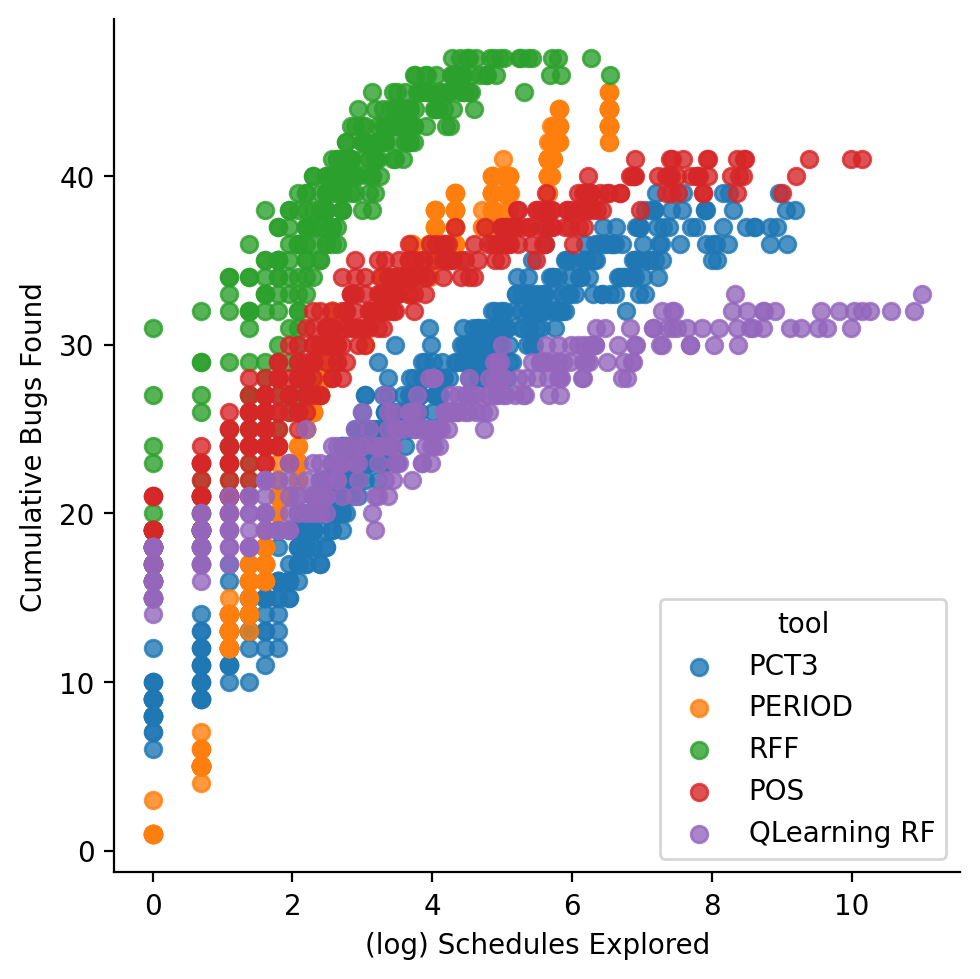
\includegraphics[width=.7\linewidth]{cum-scheds-to-bug}
    \caption{\label{fig:test1}test1}
\end{figure}

我们将前面的几种工具应用在两个基准测试上运行,衡量的标准是每一个工具在特定schedule数量下发现的漏洞数量。在这几个工作中,GenMC无法在这些基准测试上运行,因此没有放在最终的比较中。PCT找到了37个漏洞,PERIOD平均找到了44.6个bugs,而RFF平均找到了46.1个漏洞,这几乎是所有程序都成功检测到。在第47个程序的测试中,只有一部分的情况成功地找到了漏洞,因此,最终找到的漏洞平均为46.1。在图中,我们展示了每一个工具,经过一定的schedule之后,找到的漏洞的数量。这不仅反映了上面的结论,也就是RFF能比其他工具找到更多的漏洞,更反映了RFF能够在更少的schedule中找到更多的漏洞,这可以通过查看在每一个特定的schedule下,RFF几乎总是比其他的工具找到更多的漏洞。根据实验的数据,我们还可以得知,在30个程序中,RFF比PERIOD以更少的schedules找到漏洞,在9个测试程序中,Rff比PERIOD以更多的schedules找到漏洞。对于两个同样是期望通过等价类来减少探索空间的工具来说,RFF利用的reads-from relation显然能够在找到等价类上有着更好的效果。

\subsection{抽象调度在漏洞挖掘中的作用}

Rff中提出了一个新的抽象调度的概念,用来表示一个等价类,通过执行等价类中的一个具体调度,就能够测试这整个类,大大减少了探索的空间。而常规的POS中,并没有抽象调度这个概念,它是在实际的调度上进行操作的,这可能会导致其性能的不足。从图中的结果可以看到,RFF能够在相同的chedule下发现更多的漏洞,并且随着schedule的增大,发现的漏洞数量的差距也在增大。这说明,对于一些简单的容易触发的漏洞,POS也可以比较容易地挖掘,但是对于一些比较复杂的漏洞,POS即使在更多的schedule下也无法发现,而RFF值可以稳定的发现更深层次的漏洞。

\subsection{对调度空间的探索}

在对一个程序测试的过程中,如果一个调度可以有更多的reads-from relation,那么这个调度就更有可能触发程序的漏洞,因此模糊器如果能够被引导朝着更加有效的交错空间进行探索,那么就有可能发现更多的漏洞。这里测试了POS和RFF对同一个程序进行漏洞挖掘的过程中所用到的reads-from relation的数量,可以看到RFF能够检测到更多的reads-from relation,并利用这些reads-from relation产生有效的调度那行探索,相比之下,POS只能产生有限的reads-from relation。这是因为RFF在对当前的种子进行排序时,会更加倾向于那些拥有新的reads-from relation的种子,相比于POS的随机选取算法来说,这有助于模糊测试向着更有可能发现漏洞的交错空间进行探索。

\begin{figure}[ht]
    \centering
    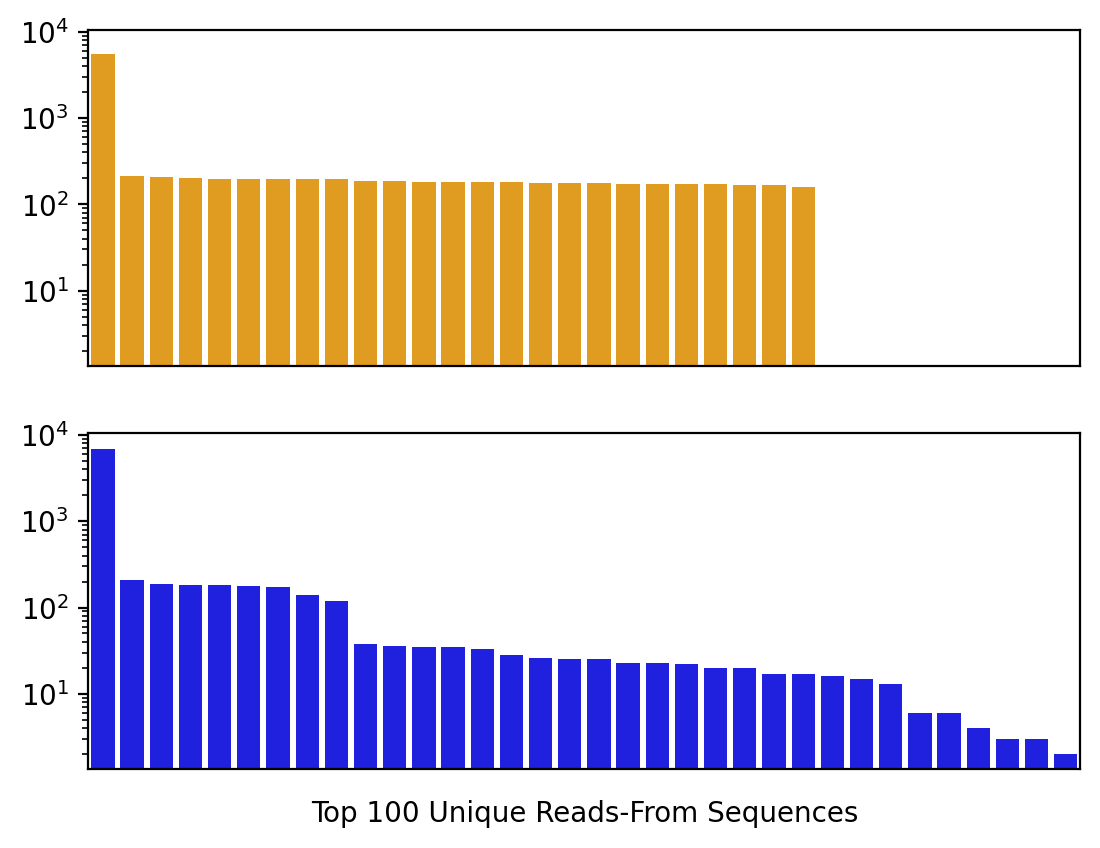
\includegraphics[width=.7\linewidth]{bar}
    \caption{\label{fig:test2}test2}
\end{figure}

\section{现有工作评估}

\subsection{当前各种工具的优劣}

\subsubsection{当前工具的介绍}

RFF的实现主要是由两个部分组成,第一个部分是调度的控制